\chapter{Understanding the dataset}\label{cap:analisis}


\section{Introduction}

This research is based on the Genomics of Drug Sensitivity in Cancer (GDSC) dataset, available through Kaggle. The primary aim of this resource is to make publicly available data from the original GDSC repository, with additional annotations to facilitate downstream analysis.

The dataset includes detailed information about various cancer cell lines and their associated types. It provides genomic and molecular features such as mutation status, tissue origin, growth conditions, and methylation patterns. On the pharmacological side, it offers drug-specific information, including treatment response, administered concentrations, and metadata related to drug selection. In addition, it includes a classification label that reflects the effectiveness of the drug response.

Among the most critical variables is the logarithm of the half-maximal inhibitory concentration, denoted as \(LN\_IC_{50}\). This metric quantifies the drug dosage required to inhibit cell viability by 50\%, making it a biologically meaningful and clinically relevant target for prediction. A model capable of accurately predicting \(LN\_IC_{50}\) could serve as a decision-support tool in assigning optimal drug dosages to individual patients. Moreover, gaining insight into the factors that influence this value could offer valuable directions for further research in personalized medicine and oncology.

\section{Description of variables}

The dataset Genomics of Drug Sensitivity in Cancer (GDSC) comprises a total of four files, each providing complementary information on the status of cancer cell lines, patient characteristics, and prescribed medications. One of the most important features of this dataset is that the information it
contains comes from the COSMIC database \cite{cosmic}, one of the most comprehensive
collections on cancer cases and their treatment. In the following sections, each file will be briefly described along with the variables it contains, in order to provide an initial understanding of their relevance and potential utility for this research.

\begin{enumerate}
    \item \textbf{GDSC2-dataset.csv}: Mainly contains information about the medicines used and their effectiveness in the different patients. Among its variables are:
    \begin{itemize}
        \item \textbf{DATASET}: Since the objective of the author of the dataset is to keep the information updated, he uses this variable to indicate which version it comes from, since the database \textit{COSMIC} is updated regularly.
        \item \textbf{NLME\_RESULT\_ID}: Unique identifier of the NLME model to which it is related.
        \item \textbf{NLME\_CURVE\_ID}: Identifier of the dose-response curve fitted by the previous model.
        \item \textbf{COSMIC\_ID}: As its name suggests, this is the identifier by which this record is known in the database \textit{COSMIC}.
        \item \textbf{CELL\_LINE\_NAME}: Name of the cancer cell line of the experiment.
        \item \textbf{SANGER\_MODEL\_ID}: Identifier of the cell used by the Sanger Institute \cite{sanger}.
        \item \textbf{TCGA\_DESC}: Description of the type of cancer according to \textit{The Cancer Genome Atlas}\footnote{Project with the aim of cataloging genomic alterations due to the presence of cancer cells.}.
        \item \textbf{DRUG\_ID}: Identifier of the drug prescribed to the patient.
        \item \textbf{DRUG\_NAME}: Name of the drug used in the treatment.
        \item \textbf{PUTATIVE\_TARGET}: Refers to the original cellular target of the drug, i.e. which cell line the drug is intended to treat.
        \item \textbf{PATHWAY\_NAME}: The biological pathway affected by the drug, i.e., which series of cellular interactions the drug intake modifies.
        \item \textbf{COMPANY\_ID}: Identifier of the company that provides the drug.
        \item \textbf{WEBRELEASE}: Date on which this information was made public on the website.
        \item \textbf{MIN\_CONC}: Minimum used concentration of the drug during follow-up.
        \item \textbf{MAX\_CONC}: Maximum drug concentration used during follow-up.
        \item \textbf{LN\_IC50}: This variable represents the natural logarithm of the $IC_{50}$ value (mean inhibitory concentration). A higher value indicates that a greater dose of the drug is required to achieve the desired effect, suggesting lower sensitivity or resistance. Conversely, a lower value implies that only a small dose was sufficient to produce a significant biological response, indicating higher sensitivity to the drug.
        \item \textbf{AUC}: Area Under the Curve, a statistical measure that in this case reflects the effectiveness of the drug.
        \item \textbf{RMSE}: Error measure known as Root Mean Square Error. It indicates the quality of the dose-response prediction performed by the NLME model.
        \item \textbf{Z\_SCORE}: Standardized performance measure, intended to allow comparisons between different drugs and cell lines.
      \end{itemize}

      \item \textbf{Cell\_Lines\_Details.xlsx}: Contains information about the different cell lines, as well as data related to the patient's cancer. The variables it includes are:
      \begin{itemize}
        \item \textbf{Sample Name}: Unique identifier for the cell line sample.
        \item \textbf{COSMIC identifier}: Unique ID from the COSMIC database for the cell line.
        \item \textbf{Whole Exome Sequencing (WES)}: Genetic mutation data obtained through whole exome sequencing.
        \item \textbf{Copy Number Alterations (CNA)}: Data on gene copy number changes in the cell line.
        \item \textbf{Gene Expression}: Information on gene expression levels in the cell line.
        \item \textbf{Methylation}: Data on DNA methylation patterns in the cell line.
        \item \textbf{Drug Response}: Information on how the cell line responds to various drugs.
        \item \textbf{GDSC Tissue descriptor 1}: Primary tissue type classification. Mainly indicates the type of cancer.
        \item \textbf{GDSC Tissue descriptor 2}: Secondary tissue type classification. It can be interpreted as indicating the region affected by cancer.
        \item \textbf{Cancer Type (matching TCGA label)}: Cancer type according to the TCGA classification.
        \item \textbf{Microsatellite instability Status (MSI)}: Indicates the microsatellite instability status of the cell line.
        \item \textbf{Screen Medium}: Growth medium used to culture the cell line.
        \item \textbf{Growth Properties}: Characteristics of how the cell line grows in culture.
        \end{itemize}

    \item \textbf{Compounds-annotation.csv}: The data in this file refer mainly to the drug:
        \begin{itemize}
            \item \textbf{DRUG\_ID}: Unique identifier for the drug.
            \item \textbf{SCREENING\_SITE}: Location where the drug screening was performed.
            \item \textbf{DRUG\_NAME}: Name of the drug compound.
            \item \textbf{SYNONYMS}: Alternative names for the drug.
            \item \textbf{TARGET}: The molecular target(s) of the drug.
            \item \textbf{TARGET\_PATHWAY}: The biological pathway(s) targeted by the drug.
        \end{itemize}

    \item \textbf{GDSC\_DATASET.csv}: This dataset is the result of preprocessing performed by the original Kaggle author, based on three raw data files included in the same repository. The author applied extensive data cleaning and transformation techniques to reduce noise, enhance signal quality, and incorporate relevant domain knowledge. The resulting file provides a curated version of the data that is ready for analysis and modeling. Among the variables included in this dataset are:
    \begin{table}[H]
        \centering
        \begin{tabular}{|l|l|}
        \hline
        \textbf{COSMIC\_ID} & \textbf{CELL\_LINE\_NAME} \\ \hline
        \textbf{TCGA\_DESC} & \textbf{DRUG\_ID} \\ \hline
        \textbf{DRUG\_NAME} & \textbf{LN\_IC50} \\ \hline
        \textbf{AUC} & \textbf{Z\_SCORE} \\ \hline
        \textbf{GDSC Tissue descriptor 1} & \textbf{GDSC Tissue descriptor 2} \\ \hline
        \textbf{Cancer Type (matching TCGA label)} & \textbf{Microsatellite instability Status (MSI)} \\ \hline
        \textbf{Screen Medium} & \textbf{Growth Properties} \\ \hline
        \textbf{CNA} & \textbf{Gene Expression} \\ \hline
        \textbf{Methylation} & \textbf{TARGET} \\ \hline
        \multicolumn{2}{|c|}{\textbf{TARGET\_PATHWAY}} \\ \hline
        \end{tabular}
        \caption{List of variables present in the GDSC dataset.}
        \label{tab:gdsc_vars}
        \end{table}
\end{enumerate}

Although the preprocessing of the GDSC\_DATASET file is very interesting, its data has not been used for this research. It eliminates some variables that were considered useful for improving the prediction results. For example, including "DRUG\_RESPONSE" among the variables to be predicted could help the model understand some internal relationships in the data. However, given that the procedures applied could be helpful in resolving this research, some of the data provided has been taken into account.


\section{Analyzing the information}

The variable of greatest interest is \(LN\_IC_{50}\), as it is the one that would allow us to know how much medication to administer to the patient. Therefore, the first step is to understand its distribution. This makes it possible to anticipate potential problems understand how it evolves.

\begin{figure}[H]
    \centering
    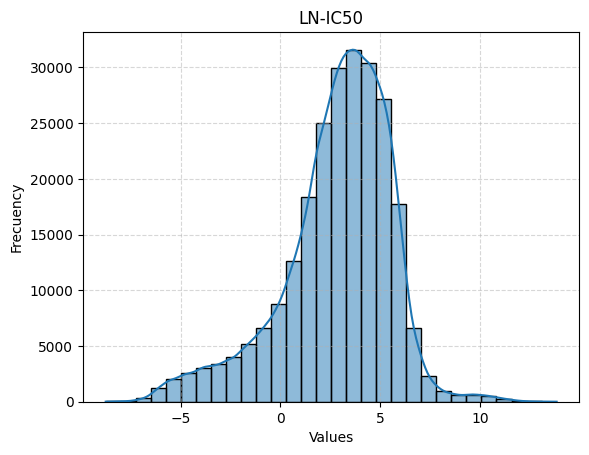
\includegraphics[width=1\textwidth]{figures/LNIC_50_barplot.png}
    \caption{Distribution of the \(LN\_IC_{50}\) variable.}
    \label{fig:lnic50_distribution}
\end{figure}

Figure~\ref{fig:lnic50_distribution} shows how the \(LN\_IC_{50}\) variable follows a normal distribution in which some aspect can be observed:

\begin{itemize}
    \item There are fewer examples on the right side of the distribution, which implies that the data has been slightly skewed when acquiring positive values.
    \item In the same area on the right, a small increase can be seen. This may indicate a population for which more records are available on an ad hoc basis, which could pose a small challenge during model training, as this population disrupts the natural progression of the normal distribution.
    \item In general, it shows good symmetry, thus favouring the training of a model, ignoring the area mentioned above.
\end{itemize}

\subsubsection{Joining the data}

Once the main target variable has been analysed, it is necessary to know how to join the files appropriately so that the records match their corresponding ones. Thus, referring to database terminology, it is necessary to carry out various join operations between the three files, relating each of the foreign keys\footnote{In the context of relational databases, it refers to an identifier that helps link records from one table to records from another.} to their corresponding primary keys.

There are unknown records in each of the three files, so there are several possibilities:
\begin{itemize}
    \item Delete all null values and perform the joins afterwards.
    \item Join the three files and apply value imputation to try to infer the value of the unknown fields.
    \item Join the datasets and then delete the resulting null values.
\end{itemize}

To obtain the complete dataset, it is necessary to merge the GDSC2 and Cell\_Lines\_Details files using  "COSMIC\_ID" and "COSMIC identifier" keys. This is because both records come from different sections of the COSMIC database. The resulting dataset must be linked to Compounds-annotation using the "DRUG\_ID" key, thus obtaining a record with all the data.

When making a decision, it is important to consider that value imputation could improve performance. However, if some of the records are deleted and assigned a status to those that are unknown, the future model could acquire a certain degree of resilience, strengthening the model. Based on this, two decisions were made. Investigate two of the possibilities: on the one hand, the datasets will be joined, applying a process of value imputation a posteriori. On the other hand, null records will be deleted and then the files will be merged. Both resulting datasets will be used in a first regressor to check which data provides the most value. Although this may seem complex, the implementation is straightforward using notebook files\footnote{Development environment that allows you to run code organized in cells}, as the two workflows are nearly identical except for the step involving imputation. This approach will be detailed in a subsequent section.

\subsubsection{Filtering the information}

Applying variable selection procedures reduces the dimensionality of the dataset. This has two key benefits: on the one hand, it reduces noise in the dataset and lowers the computational cost of training the model. On the other hand, it reduces the potential of human error during the initial data collection process. In practical terms, if you only need to record 10 characteristics instead of 20, the likelihood of introducing mistakes during data entry or measurement is significantly lowered.

The current dataset contains many identifiers related to external studies or various databases. These identifiers will not be necessary for this research, meaning that these variables are disposable.

\begin{itemize}
    \item DATASET
    \item NLME\_CURVE\_ID
    \item COMPANY\_ID
    \item COSMIC identifier
    \item Sample Name
    \item COSMIC\_ID
    \item SYNONYMS
\end{itemize}

The next step is to check if any of the variables are obsolete. This condition occurs when all available records for that feature are always the same. To do this, the code described in Listing~\ref{cod:obsoletes} has been used. This makes it possible to identify obsolete variables and determine the size of each variable's domain.

Apparently, the DRUG\_ID and DRUG\_NAME variables contain the same information, so one of them could be discarded. To be sure, it is necessary to check whether there are any inconsistencies in the data and, if so, to determine whether this is due to an error during data collection or whether the information provided is actually important. To check consistency, the function illustrated in Listing~\ref{cod:inconsistencesNameId} has been used. This code systematically scans the dataset to confirm that each drug ID matches its corresponding drug name. In cases where mismatches are detected, the function attempts to identify which variable is inconsistent, providing insight into the source of the discrepancy.

This reveals that there is inconsistency in the names, i.e. some names correspond to more than one identifier. To understand the nature of this inconsistency, the identifiers of the suppliers of these drugs are examined, as they may have a different identifier depending on the supplier. To do this, the code visible in Listing~\ref{cod:supplierConsistence} is used.

\begin{table}[H]
    \centering
    \begin{tabular}{|l|l|l|}
    \hline
    \textbf{Drug Name} & \textbf{Detected IDs} & \textbf{Supplier IDs} \\ \hline
    Docetaxel & [1007, 1819] & [1046, 1043] \\ \hline
    Selumetinib & [1062, 1736] & [1046, 1001] \\ \hline
    Oxaliplatin & [1089, 1806] & [1046, 1043] \\ \hline
    Fulvestrant & [1200, 1816] & [1046, 1043] \\ \hline
    Uprosertib & [1553, 2106] & [1046] \\ \hline
    GSK343 & [1627, 2037] & [1046, 1033] \\ \hline
    Acetalax & [1803, 1804] & [1043] \\ \hline
    Dactinomycin & [1811, 1911] & [1043, 1046] \\ \hline
    Ulixertinib & [1908, 2047] & [1046] \\ \hline
    \end{tabular}
    \caption{Detected inconsistencies between DRUG\_NAME, DRUG\_ID, and their suppliers}
    \label{tab:drug_id_supplier}
\end{table}

Table~\ref{tab:drug_id_supplier} shows that, with the exception of three cases, in all others, when there is an inconsistency between the drug name and its identifier, the medicine is supplied by a different provider. This information can be very useful, as variations between suppliers may involve subtle changes to some component of the drug formula, its preservation or concentration. Therefore, the Drug name and Drug id variables will be retained in the dataset, while the company identifier will be omitted.

\subsubsection{Modifying the representation of data}

Many operations, such as computing correlations, visualizing data, or training machine learning models, require the dataset to be in a numerical format. Therefore, the next step involves transforming categorical variables into numerical representations. A common technique is one-hot encoding; however, this method significantly increases the dimensionality of the dataset, which may negatively affect performance and training time. As an alternative, ordinal encoding will be applied where appropriate, allowing the numerical representation to preserve the inherent order or semantic relationships of the original categories. For example, in a variable representing size with values such as \textit{small}, \textit{medium}, and \textit{large}, assigning them the values 0, 1, and 2, respectively, maintains their natural ordering.

The following variables only express information of Yes, No or unknown value, making them clear candidates for replacement.
\begin{itemize}
    \item Copy Number Alterations (CNA)
    \item Gene Expression
    \item Methylation
    \item Drug Response
\end{itemize}

The Growth Properties variable contains information regarding adhesion, differentiated into three levels: Adherent, Semi-Adherent, and Suspension. Therefore, applying a numerical substitution indicating the degree of adhesion is a plausible option.

Finally, the Screen Medium variable only takes two values, "R" and "D/F12", so instead of applying one-hot encoding, it can be encoded as 0 or 1, depending on which option it is.

In order to facilitate the application of these changes to future data, this entire process is carried out using Sklearn's ColumnTransformer. This class allows you to perform a sequence of transformations on the data easily and effectively. The steps required to do this are illustrated in Listing~\ref{cod:columnTransformer}.

\subsection{Checking the feasibility of assigning values}

The imputation of unknown values could improve results, which is why research has been conducted on this topic. The objective is to conduct a small test to verify whether imputing values improves accuracy or whether, on the contrary, allowing a certain degree of ambiguity in the data improves the robustness of the model. To achieve this, the steps described below have been followed.

To perform the imputation process, all variables must be numbers. However, after the preprocessing described above, the dataset retains some categorical features. Since these variables cannot be expressed in numerical format while maintaining the relationship between them, the ideal solution would be to apply a one-hot encoder, but this would significantly increase the computational cost of applying value imputation. Therefore, Sklearn's ordinal encoder \cite{scikit-learn-ordinalencoder} has been used, which allows categorical variables to be replaced by numerical ones, while maintaining the correspondence stored, in case it needs to be restored later. This process can be observed in Listing~\ref{cod:ordinalEncoder}.

Once the dataset does not contain categorical information, it is possible to apply imputation methods. During this research, the method selected was KNNImputer \cite{scikit-learn-knnimputer}, which creates clusters between the data and imputes values based on the nearest centroids. In other words, it assigns values based on their similarity to known data. The application of this technique can be seen in Listing~\ref{cod:knnImputer}.

\subsubsection{Comparing results}

Comparing the results between applying value imputation and assigning values to nulls after the unification process will allow us to determine which method is best for the research.

To perform the comparison, a neural network architecture consisting of three fully connected (dense) layers was implemented, as detailed in Listing~\ref{cod:pythonGenerateNet}v. This structure was chosen to ensure a fair and consistent baseline for evaluating the impact of preprocessing. The network was trained using both datasets, one with imputed values and one without. The results from each training scenario were then collected and analyzed to assess the influence of the imputation step on model performance.

\begin{table}[H]
    \centering
    \begin{tabular}{|c|c|}
    \hline
    \textbf{Metric} & \textbf{Value} \\
    \hline
    MSE  & 0.843 \\
    RMSE & 0.918 \\
    MAE  & 0.674 \\
    \hline
    \end{tabular}
    \caption{Model performance in the test set after applying value imputation.}
    \label{tab:model_metrics_imputing_values}
\end{table}

\begin{table}[H]
    \centering
    \begin{tabular}{|c|c|}
    \hline
    \textbf{Metric} & \textbf{Value} \\
    \hline
    MSE & 0.320 \\
    RMSE & 0.566 \\
    MAE & 0.300 \\
    \hline
    \end{tabular}
    \caption{Model performance in the test set without applying value imputation.}
    \label{tab:test_metrics_without_values_imputation}
\end{table}

As can be seen in Tables~\ref{tab:model_metrics_imputing_values} and \ref{tab:test_metrics_without_values_imputation}, the model's performance is severely compromised after applying value imputation. Everything seems to indicate that adding some ambiguity to the data does indeed make the model more robust and versatile.
